\documentclass[14pt]{extarticle}
\usepackage{graphicx}
\usepackage{amsmath}
\usepackage{xcolor}





\begin{document}

\title{Organizzazione e Gestione per lo startup Aziendale}
\author{Alessandro Savioli}
\date{Febbraio 2025}

\maketitle

\tableofcontents

\newpage

\section{Lezione 1}

\section{Lezione 2}

\section{Lezione 3}
\subsection{La Struttura Organizzativa}

\textbf{Organizzare} significa ordinare un sistema di parti dipendenti tra loro,
definendo per ognuna uno specifico ruolo all'interno del sistema stesso.

Per fare ciò, serve trovare una \textcolor{red}{Struttura Organizzativa}, in cui
possiamo trovare:
\begin{enumerate}
    \item Un insieme di relazioni tra le persone interne all'azienda;
    \item Una distribuzione delle Autorità e delle Responsabilità;
    \item Un insieme di processi con i quali l'azienda si costituisce.
\end{enumerate}
Questa struttura non può essere formulata partendo da un modello ideale ed
astratto, bensì deve essere \textbf{adattata} alla realtà nella quale l'azienda
opera.

Una struttura organizzativa è composta da elementi:
\begin{itemize}
    \item \textbf{Hardware (o di struttura)} meccanismo attraverso il quale
    vengono affidate delle funzioni a tutte le parti del sistema;
    \item \textbf{Software (o decisionali)} che stabilisce scopo, finalità e \\
    obiettivi dell'organizzazione e ne elabora le norme e le relazioni delle
    parti.  
\end{itemize}
Inoltre, una struttura organizzativa può essere di tipo:

\begin{itemize}
    \item \textbf{Formale}, dove la divisione in mansioni e la loro integrazione
    è esplicitamente riconosciuta e può essere rappresentata tramite gli
    \textbf{organigrammi};
    \item \textbf{Informale}, che fa riferimento a rapporti spontanei e a
    fattori di influenza e potere. 
\end{itemize}

\subsection{Gli Organigrammi}

Gli organigrammi sono delle rappresentazioni grafiche globali, di facile
comprensione, della struttura organizzativa formale dell'impresa.

Il loro scopo è quello di evidenziare gli aspetti fondamentali del funzionamento
dell'organizzazione, le posizioni strutturali ed i collegamenti tra le diverse
funzioni aziendali.
\begin{center}
    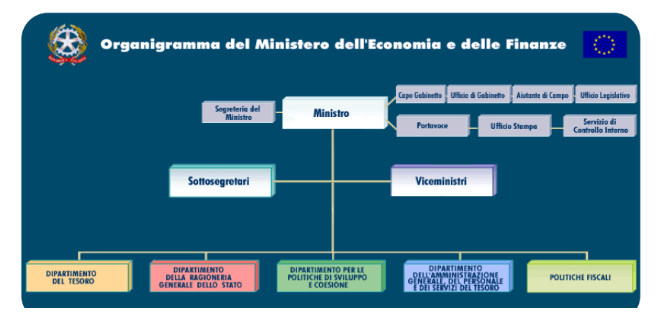
\includegraphics[scale = 0.80]{images/Esempio_Organigramma}
    Esempio di un organigramma 
\end{center}
Questo tipo di rappresentazione grafica ha però dei difetti, in quanto si fa
difficoltà a capire l'importanza delle posizioni rappresentate, non si hanno
informazioni sui rapporti non gerarchici e non si capisce in che ambiente opera
l'azienda.

\subsection{I vari Tipi di Struttura Organizzativa}
\subsubsection{Il modello Gerarchico (Struttura Monofunzionale)}

\begin{center}
    \textcolor{red!50}{CARATTERISTICHE}
\end{center}


\begin{itemize}
    \item \textbf{Principio di gerarchia}, secondo il quale \\ autorità,
    responsabilità e le competenze sono massime al vertice dell'organizzazione;
    \item \textbf{Principio di delega}, secondo il quale le funzioni vengono
    delegate verso il basso;
    \item \textbf{Principio di eccezione}, secondo il quale, in caso di
    difficoltà impreviste il problema deve tornare al vertice per essere
    risolto;
    \item \textbf{Principio dell'unità di direzione}, secondo il quale ciascuno
    deve aver ben chiaro da chi prendere ordini e a chi rivolgersi quando non
    sia in grado di decidere da solo.  
\end{itemize}

\begin{center}
    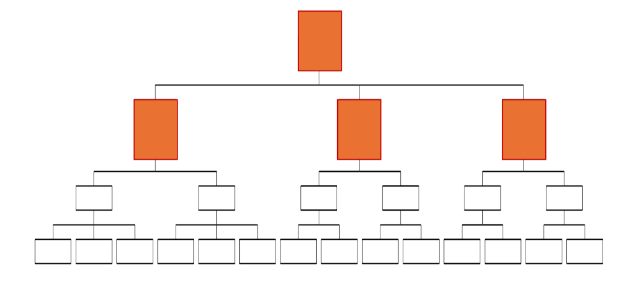
\includegraphics[scale = 0.80]{images/modello_gerarchico}
    Esempio di modello gerarchico
\end{center}

\newpage

\subsubsection{Il modello Gerarchico Funzionale (Struttura Gerarchico Funzionale)}

\begin{center}
    \textcolor{red!50}{CARATTERISTICHE}
\end{center}

Questo modello presenta attività raggruppate in base ad una funzione comune ed
esalta il \textbf{principio della specializzazione} delle singole aree.

Continua a seguire il \textbf{Principio di gerarchia} ed il \textbf{Principio di
eccezione} dal modello precedente.

\begin{center}
    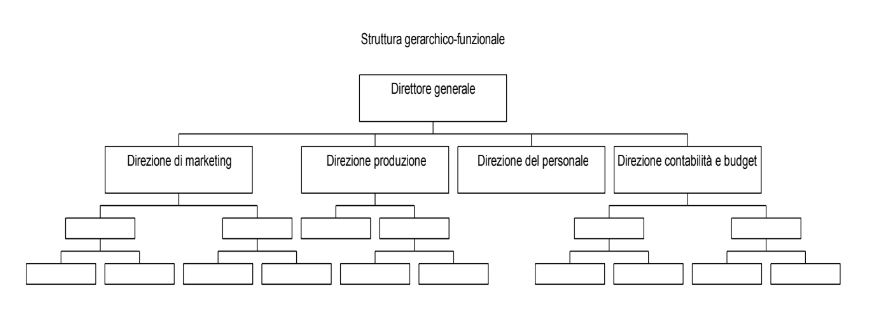
\includegraphics[scale = 0.64]{images/modello_gerarchico_funzionale}
    Esempio di modello gerarchico funzionale
\end{center}
Nella struttura gerarchico funzionale esistono tre livelli organizzativi
fondamentali:

\begin{enumerate}
    \item \textbf{Direzione generale}, a cui è affidato il compito di
    amministrare l'azienda tramite una visione d'insieme che permetta di
    definire gli obiettivi primari e coordinare le diverse aree funzionali;
    \item \textbf{Direzioni dei dipartimenti funzionali}, che sono specializzate
    nelle varie funzioni, quindi non in grado di occuparsi di problemi generali,
    ma solo di problemi settoriali;
    \item \textbf{Unità operative}, ovvero organi che fanno capo ai dipartimenti
    funzionali, per realizzare piani predisposti da quest'ultimi, hanno compiti
    prevalentemente esecutivi. 
\end{enumerate}

Le principali direzioni funzionali sono:

\begin{itemize}
    \item \textbf{Direzione Marketing};
    \item \textbf{Direzione della Produzione};
    \item \textbf{Direzione del Personale};
    \item \textbf{Direzione Amministrativa};
    \item \textbf{Direzione Finanza};
    \item \textbf{Direzione Ricerca e Sviluppo};
\end{itemize}

un esempio di modello gerarchico funzionale può essere identificato nel modello
strutturale utilizzato da Apple.

\subsubsection{Il modello Divisionale}

In questo modello vengono organizzate divisioni separate, ciascuna è
responsabile di un singolo prodotto, servizio o programma principale. Questa
struttura è anche denominata \textbf{struttura per prodotto}.

\begin{center}
    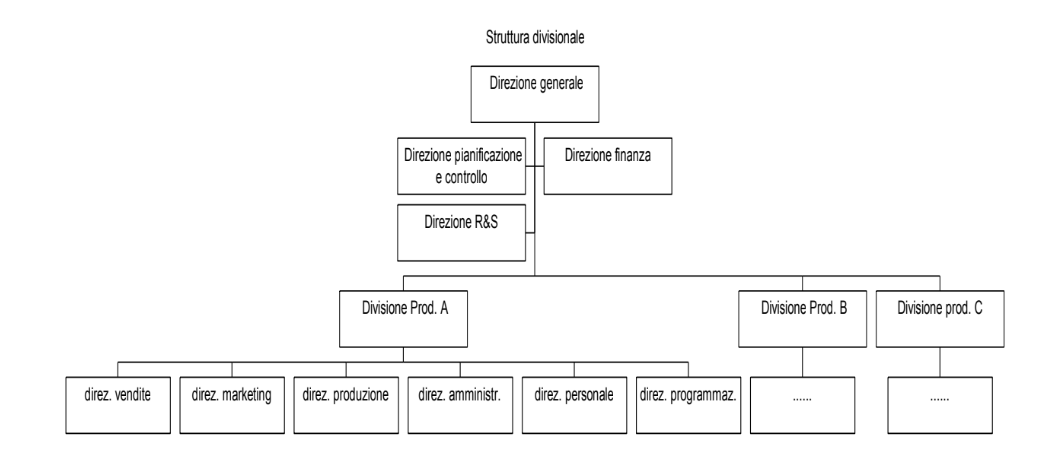
\includegraphics[scale = 0.50]{images/modello_divisionale.png}
    Esempio di modello divisionale
\end{center}

Un'azienda che adopera il modello divisionale è \textbf{Alphabet}, proprietaria
di Google.

\subsubsection{Il modello per Area Geografica}

Questo modello risulta simile al modello divisionale, con l'unica differenza che
le divisioni sono organizzate per area geografica. Questo tipo di struttura
aiuta l'azienda ad espandersi in nuovi mercati e a fare un uso più efficiente
delle risorse.

\begin{center}
    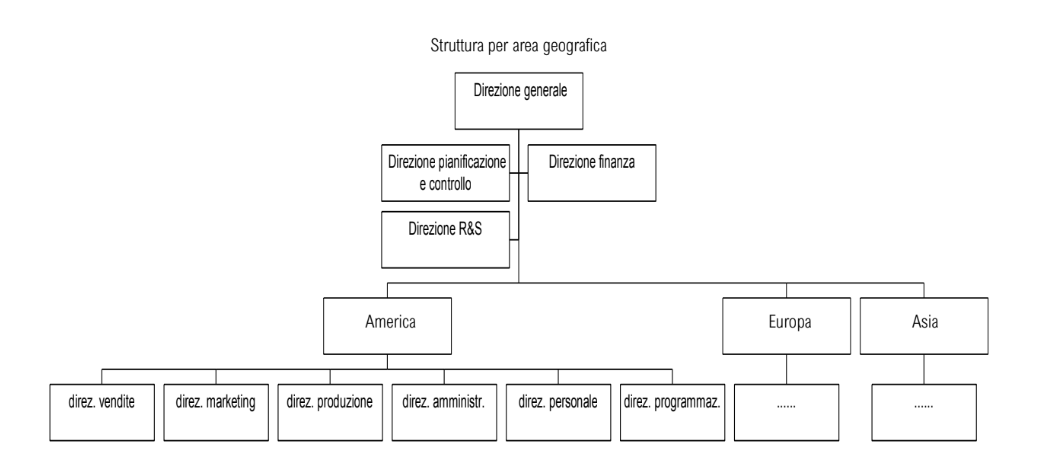
\includegraphics[scale=0.50]{images/modello_geografico.png}
    Esempio di modello per area geografica
\end{center}

\subsubsection{Il modello a Matrice}

Questo modello cerca di combinare al meglio i vantaggi dell' \\ 
organizzazione per funzioni con quelli dell'organizzazione per prodotti o
progetti.

\begin{center}
    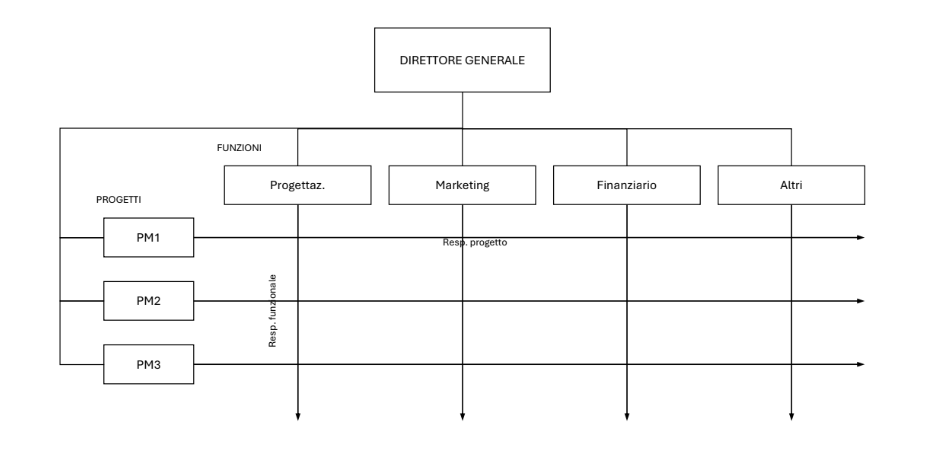
\includegraphics[scale=0.60]{images/modello_matrice.png}
    Esempio di modello a matrice
\end{center}
Molte aziende adoperano questo tipo di struttura, tra le più celebri troviamo
Intel, Spotify, Microsoft, IBM, Philips.

\subsubsection{Il modello a Rete}

Questo modello affida varie parti dell'organizzazione a partner esterni. In
questo caso si parla di \textbf{Outsourcing}, ovvero quando l'azienda ricorre a
fornitori esterni per determinati compiti o funzioni, quali la produzione, le
risorse umane o la gestione dei crediti.

\begin{center}
    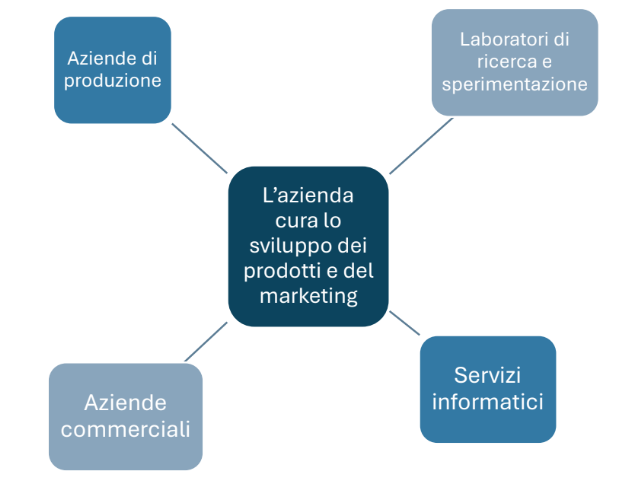
\includegraphics[scale=0.80]{images/modello_rete.png}
\end{center}
Un grande esempio di azienda che adopera questa struttura è Nike, che affida la
produzione e la distribuzione dei propri prodotti ad aziende esterne.

\section{Lezione 4}

\subsection{Stadi dello Sviluppo di un'azienda}

In questo capitolo andremo ad osservare i vari stadi dello sviluppo di
un'azienda, le varie crisi e le soluzioni che vengono adottate per poter
progredire.

\subsubsection{Stadio imprenditoriale}

Quando un'impresa è ancora allo stato embrionale, l'enfasi è posta sulla
\textbf{creazione} di un prodotto o un servizio e sulla \textbf{sopravvivenza}
nel mercato. L'organizzazione in questo momento risulta informale e non
burocratica, vi è un controllo diretto da parte del proprietario.

\begin{center}
    \textcolor{red!50}{Crisi: Bisogno di leadership}

    man mano che l'organizzazione cresce con l'aumento del numero dei dipendenti
    vengono a crearsi problemi relativi alla gestione, gli imprenditori si
    trovano costretti ad adattare una struttura organizzativa per assecondare un
    processo continuo di crescita.
\end{center}

\subsubsection{Stadio della collettività}

Se la crisi di leadership viene superata, si ottiene una direzione forte e
inizia lo sviluppo di obiettivi e di una direzione chiara dell'azienda. Vengono
strutturate le unità organizzative insieme ad una gerarchia di autorità, vengono
definiti i compiti e una prima divisione del lavoro. In questo stadio i
dipendenti cominciano ad \textbf{identificarsi} nella missione
dell'organizzazione ed idealmente dedicano molto tempo a contribuire al successo
organizzativo. La comunicazione e il controllo continuano ad essere
prevalentemente informali, comincia a nascere qualche sistema formale

\begin{center}
    \textcolor{red!50}{Crisi: Bisogno di delega}

    se il management ha operato con successo, i dipendenti a livelli inferiori
    si trovano limitati dalla forte leadership esercitata dall'alto, d'altra
    parte i manager di livello inferiore cominciano a chiedere una maggiore
    fiducia, l'organizzazione si trova dunque a dover escogitare un meccanismo
    per coordinare le diverse unità senza la supervisione del vertice.
\end{center}

\subsubsection{Stadio della formalizzazione}

Vengono introdotte nuove regole, procedure e sistemi di controllo. La
comunicazione diviene formale e segue la linea gerarchica. La direzione comincia
ad interessarsi maggiormente a strategia e pianificazione lasciando gli aspetti
produttivi ad un livello più basso di management.

\begin{center}
    \textcolor{red!50}{Crisi: Eccesso di burocrazia}

    Lo sviluppo dell'organizzazione porta ad una proliferazione di sistemi e
    procedure che possono cominciare a soffocare i manager dei livelli
    intermedi. L'organizzazione risulta troppo grande e complessa per essere
    gestita da programmi formali.
\end{center}

\subsubsection{Stadio di elaborazione}

La soluzione all'ultima crisi consiste nel far raggiungere alla burocrazia il
suo limite superiore (oltre il quale avremmo un eccesso), i manager imparano a
lavorare all'interno della burocrazia senza doverla accrescere. In questi casi
l'azienda può anche essere scomposta in divisioni per mantenere la filosofia da
piccola azienda.

\begin{center}
    \textcolor{red!50}{Crisi: Bisogno di rivitalizzazione}

    Dopo che l'azienda ha raggiunto la maturità è possibile che si cominci a
    manifestare un bisogno di rinnovamento, che può essere sentito con cadenze
    che vanno dai 10 ai 20 anni. L'azienda si disallinea rispetto all'ambiente
    in cui opera o diventa lenta e troppo burocratica, deve passare attraverso
    uno stadio di snellimento e innovazione.
\end{center}

\begin{center}
    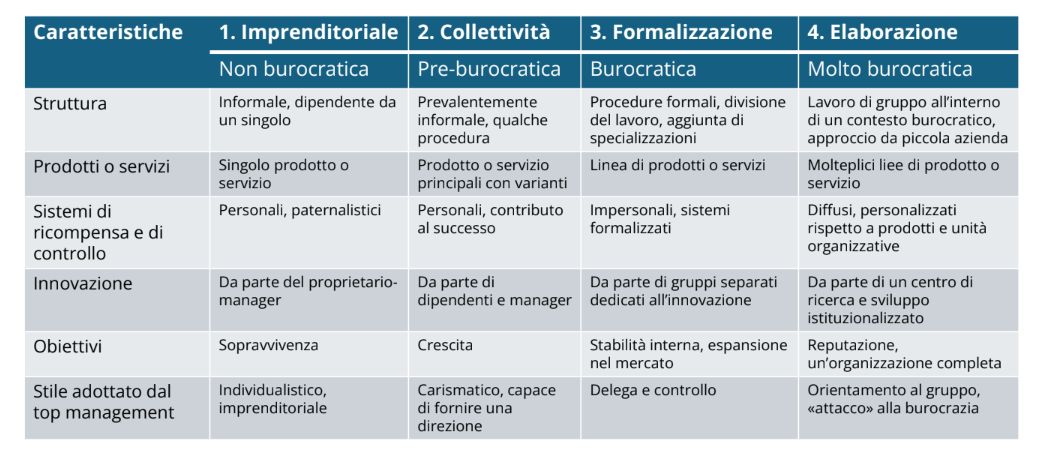
\includegraphics[scale=0.50]{images/stati_sviluppo.png}
    Mappa degli stadi di sviluppo
\end{center}

\subsection{Stadi del Declino di un'azienda}

Sulla base di un ampio studio sul declino organizzativo è stato \\
proposto un modello che attraversa 5 stadi fino alla \textbf{dissoluzione}
dell'organizzazione.

\subsubsection{Stadio della cecità}

Essendo il primo stadio, risulta complesso per il management avvertire i segnali
di declino, che possono presentarsi sotto forma di:

\begin{enumerate}
    \item Personale in eccesso;
    \item Procedure troppo complesse;
    \item Mancanza di allineamento con il proprio target;
    \item Ecc. 
\end{enumerate}
La soluzione per prevenire questo stato di \textbf{cecità} è mettere \\ in campo
sistemi di monitoraggio e di controllo che indichino prontamente quando qualcosa
non funziona, infatti potendo contare su informazioni tempestive il management
può riportare l'organizzazione alle prestazioni ottimali.

\subsubsection{Stadio dell'inattività}

Questo stadio deriva da una mancata attenzione alle condizioni correnti di
declino malgrado eventuali segni di calo delle prestazioni. La soluzione per
prevenire l'\textbf{inattività} è riconoscere l'eventuale declino e
intraprendere azioni rapide per riallineare l'organizzazione. Queste azioni
possono comprendere:

\begin{enumerate}
    \item Nuovi approcci alla risoluzione dei problemi;
    \item Maggiore partecipazione al processo decisionale;
    \item Incoraggiamento delle manifestazioni di insoddisfazione da parte dei
    dipendenti e dei clienti per capire cosa non funziona.   
\end{enumerate}

\subsubsection{Stadio dell'errore}

In questo stadio l'organizzazione affronta i problemi gravi e gli indicatori che
mostrano che i cattivi risultati non possono più essere ignorati. Il management
è quindi costretto a ricorrere a cambiamenti drastici.

Le possibilità per far fronte a questa situazione possono essere:

\begin{enumerate}
    \item Ridurre i costi, tagliando il personale;
    \item Ridurre l'incertezza dei dipendenti chiarendo valori e fornendo
    informazioni;  
\end{enumerate}

Un errore commesso in questo stadio può sancire il \textbf{punto di non ritorno}
per l'organizzazione.

\subsubsection{Stadio della crisi}

A questo punto non si è stati ancora in grado di gestire in modo efficace il
declino e ci si trova in una situazione di panico. L'unica soluzione è una
\textbf{radicale riorganizzazione}. Vengono intraprese soluzioni drastiche, come
la sostituzione del management, rivoluzioni a livello di struttura, strategia e
cultura. In questo caso il taglio della forza lavoro può essere molto severo.

\subsubsection{Stadio della dissoluzione}

Questo stadio risulta irreversibile. L'organizzazione subisce perdite ingenti di
quote di mercato e di reputazione, dei suoi migliori talenti e dei capitali.
L'unica azione possibile è quella di porre fine all'organizzazione in maniera
ordinata.

\begin{center}
    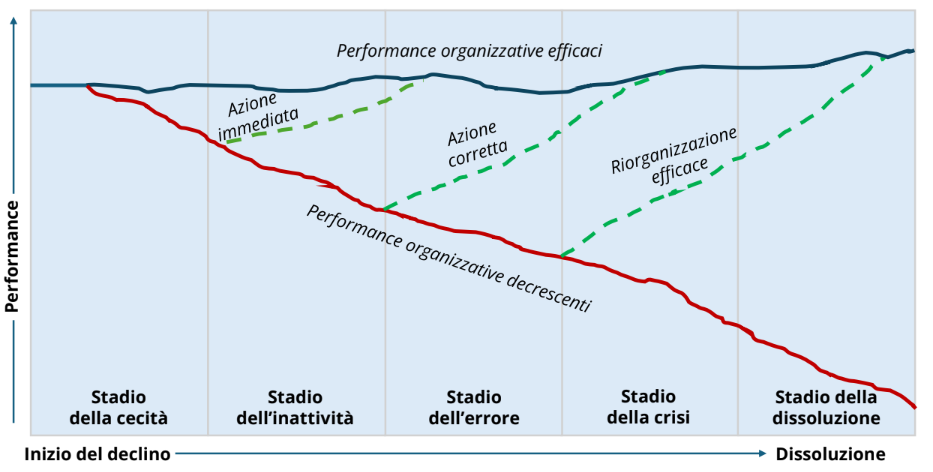
\includegraphics[scale=0.60]{images/stadi_declino.png}
    Mappa degli stadi del declino
\end{center}

\newpage
\subsection{I diversi tipi di Azienda in Italia}

Secondo l'articolo 2555 del codice civile l'azienda è \textbf{il complesso dei
beni organizzati dall'imprenditore per l'esercizio dell'impresa}. Vediamo
insieme due tipi di azienda:

\begin{itemize}
    \item \textbf{Aziende di produzione (imprese profit)}, che rendono \\
    disponibili i loro prodotti o servizi per il consumo o per altre imprese
    mediante lo scambio di mercato; 
    \item \textbf{Aziende di erogazione (corporazioni, fondazioni)}, che
    soddisfano i bisogni di determinati soggetti (associati, affiliati,
    fondatori) direttamente.
    \begin{itemize}
        \item \textbf{Corporazioni}, in cui è prevalente l'elemento personale.
        Mediante la raccolta dei contributi degli associati riescono a
        soddisfare i propri bisogni;
        \item \textbf{Fondazioni}, in cui è prevalente l'aspetto patrimoniale.
        Sorgono in virtù di lasciti o donazioni per raggiungere determinati
        scopi individuali e di utilità sociale. 
    \end{itemize} 
\end{itemize}

\subsubsection{La ditta individuale o società}

Le aziende di produzione possono essere esercitate in:

\begin{itemize}
    \item \textbf{Forma individuale}
    \item \textbf{Forma collettiva, ovvero in società} 
\end{itemize}

\newpage
Nella \textbf{Ditta individuale} il titolare risponde illimitatamente delle
obbligazioni contratte dall'azienda, indipendentemente dalla parte del suo
patrimonio investita nella ditta stessa.

\begin{center}
    \textbf{Vantaggi}:

    imposizione fiscale unica, contabilità semplice, gestione poco costosa.

    \textbf{Svantaggi}:

    Responsabilità illimitata.
\end{center}

Secondo l'articolo 2247 del codice civile:
\begin{center}
    \textbf{con il contratto di società due o più persone conferiscono beni o
servizi per l'esercizio comune di un'attività economica allo scopo di dividerne
gli utili}
\end{center}

Abbiamo due tipi di società differenti:

\begin{itemize}
    \item \textbf{Società di persone}, come s.s., s.n.c., s.a.s., che hanno una
    gestione poco onerosa ma allo stesso tempo hanno una responsabilità
    economica illimitata;
    \item \textbf{Società di capitali}, come s.p.a., s.a.p.a., s.r.l., s.r.l.s,
    che hanno una responsabilità \\
    limitata ma per questo ottengono un'imposizione fiscale doppia, con
    conseguente gestione onerosa. 
\end{itemize}

\subsection{Il bilancio di un'azienda}

Il bilancio d'esercizio è un documento informativo per un insieme eterogeneo di
soggetti, risulta utile per determinare il reddito d'esercizio e il capitale di
funzionamento, ovvero darci un'idea di come stia andando l'azienda.

TUTTE le aziende sono obbligate a redigere annualmente il bilancio ma con
modalità differenti:

\begin{itemize}
    \item \textbf{Società di capitali}: Il bilancio deve essere compilato
    seguendo uno schema a struttura obbligatoria e deve essere reso pubblico; 
    \item \textbf{Società di persone}: Il bilancio può essere presentato in
    forma libera e non è soggetto a pubblicazione. 
\end{itemize}

\subsubsection{Elementi di un bilancio d'esercizio}

Il bilancio di esercizio di una società è composto dai seguenti elementi:

\begin{enumerate}
    \item Lo \textbf{Stato patrimoniale};
    \item Il \textbf{Conto economico};
    \item La \textbf{Nota integrativa}.
\end{enumerate}

Lo \textcolor{red}{stato patrimoniale} rappresenta la situazione patrimoniale e
finanziaria della \\
società. In quest'ultimo vengono indicate le attività, passività e il patrimonio
netto della società alla data di chiusura dell'esercizio.

Il \textcolor{red}{conto economico} evidenzia il risultato economico
dell'esercizio, fornisce una rappresentazione delle operazioni di gestione,
sintetizzando componenti positivi e negativi di reddito che hanno contribuito al
risultato economico.

La \textcolor{red}{nota integrativa} costituisce parte integrante del bilancio,
fornendo informazioni aggiuntive ai dati presenti nei due punti precedenti.

\newpage
\subsection{l'Analisi di bilancio}

L'analisi di bilancio serve a monitorare lo stato di salute di un'impresa. Per
potere analizzare correttamente un bilancio, serve prima
\textbf{riclassificarlo}, per poter:

\begin{enumerate}
    \item Rendere omogenei i dati di bilancio;
    \item far emergere alcune informazioni non immediate.
\end{enumerate}

\section{Lezione 5}

\subsection{La start-up}

Unendo le definizioni date da \textbf{Eric Ries}, \textbf{Paul Graham} e
\textbf{Steve Blank} possiamo introdurre la start-up come un'azienda giovane,
innovativa, rapida, scalabile, replicabile, sostenibile e attuabile.

Ogni impresa ha una sua fase di start-up, ovvero un periodo nella prima fase di
vita in cui si definiscono i processi organizzativi e gli investimenti
economici.

\begin{center}
    \textcolor{red!50}{Differenza tra impresa e start-up}
\end{center}
Possiamo notare come la prima non ha tendenzialmente un'attività imprenditoriale
scalabile (si pensi all'apertura di un ristorante o una palestra), mentre la
seconda si fonda su un \textbf{progetto innovativo e scalabile}, ovvero
replicabile in dimensioni sempre più grandi, con profitti crescenti per
trasformarsi in una grande impresa in \textbf{tempi rapidi}.

\newpage
\subsection{La Hockey Stick Growth}

Un immagine utile a comprendere la velocità di crescita di una start-up è
proprio quella di una mazza da hockey, che rende immediato capire il concetto di
\textbf{crescita esponenziale}.

\begin{center}
    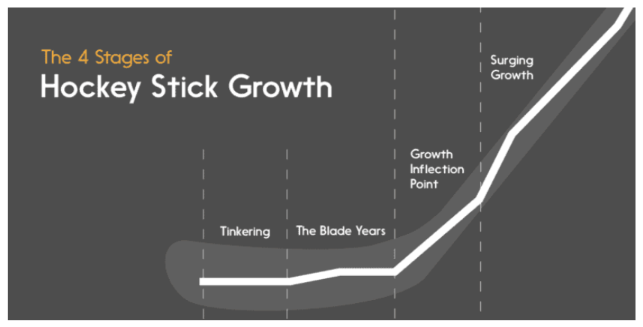
\includegraphics[scale=0.80]{images/hockey_stick.png}
\end{center}
Gli stadi principali di questa crescita sono:
\begin{itemize}
    \item \textbf{Tinkering stage};
    \item \textbf{The blade years};
    \item \textbf{Growth inflection point};
    \item \textbf{Surging growth}.   
\end{itemize}
Andiamo ora a studiarli singolarmente.

\newpage
\subsubsection{Tinkering stage, fase di avvio}

In questa fase gli imprenditori devono capire se la loro idea sia fattibile,
cercando anche di trovare il giusto equilibrio tra problemi e soluzioni. Il
tinkering termina quando si passa dalla teoria alla pratica.

Anche se questa fase non comporta molta pressione agli imprenditori, ci sono due
errori principali che potrebbero comunque mandare all'aria un'idea innovativa,
quali:

\begin{enumerate}
    \item Perdere troppo tempo nella costruzione di un business model accurato;
    \item Non cercare feedback sul prodotto/servizio per paura che l'idea venga
    copiata. 
\end{enumerate}
In questo momento l'attenzione deve essere rivolta alla sperimentazione e allo
sviluppo dell'offerta in base ai feedback ricevuti dai potenziali clienti.

\subsubsection{Blade years stage, fase di trazione}

I Blade years sono il periodo di tempo in cui viene convalidata l'idea sul
mercato, utilizzando versioni grezze, come l'MVP (Minumum Valuable Product) o la
versione beta, e in cui viene sviluppata l'idea finale e il relativo modello di
business. Solitamente in questa fase viene attuato il cosidetto
\textbf{bootstrapping}, ovvero cercare round d'investimenti per poter finanziare
il progetto. Ecco eventuali errori che un imprenditori potrebbe commettere
durante i blade years:

\begin{enumerate}
    \item Dedicare troppo tempo a raccogliere capitali per pagare le spese
    personali;
    \item Spendere troppo per le attività di vendita e marketing;
    \item Non essere disposti a modificare ulteriormente il prodotto.  
\end{enumerate}

\subsubsection{Growth inflection point, fase di scalabilità}

Qui ci troviamo al punto di svolta, il business model viene perfezionato e le
entrate dovrebbero cominciare a crescere in modo esponenziale. Gli imprenditori
possono sfruttare il loro slancio di crescita per attirare \textbf{venture
capitalist} o altri investitori.

Questa fase però presenta rischi significativi:

\begin{enumerate}
    \item Non riuscire a controllare la crescita dell'attività potrebbe \\
    portare ad un crollo;
    \item Pensando di sfruttare al massimo l'opportunità di crescita, si tende a
    modificare un prodotto che ha già funzionato fino a questo momento. 
\end{enumerate}
L'obiettivo principale deve essere quello di valutare attentamente le operazioni
e di sincronizzarle con la crescita dei ricavi.

\subsubsection{Surging growth stage, fase di maturità}

Una volta che la start-up si dimostra capace di sostenere la crescita
esponenziale durante lo stadio precedente, la sua crescita continua ad
accellerare a ritmo sostenuto, attirando sempre più clienti a provare l'offerta.

In questa fase, gli imprenditori devono affrontare le difficoltà che derivano
dall'esplosione di mercato, per questo si trovano davanti a tre scelte:

\begin{enumerate}
    \item Vendere l'azienda;
    \item Rimanere l'amministratore delegato;
    \item Assumere un amministratore delegato per gestire l'azienda. 
\end{enumerate}

\subsection{La start-up in Italia}

Nell'ordinamento giuridico in Italia è riconosciuta la \textbf{start-up
innovativa}. Queste start-up devono soddisfare almeno uno dei tre seguenti
punti:

\begin{enumerate}
    \item Almeno il 15\% del maggiore tra fatturato e costi annui deve essere
    rivolto ad attività di \textbf{ricerca e sviluppo};
    \item La forza lavoro è costituita per almeno un terzo da dottorandi, oppure
    da almeno due terzi da soci o collaboratori in possesso di laurea
    magistrale;
    \item L'impresa è titolare di un \textbf{brevetto o software registrato}.  
\end{enumerate}
Sono previsti incentivi per chi investe nelle start-up. Le persone fisiche hanno
il diritto a detrarre un importo pari al 30\% dell'investimento con un limite
massimo di 1 milione di euro annui, con un periodo minimo di mantenimento
dell'investimento pari a 3 anni.

Le società ottengono la stessa percentuale, con le stesse condizioni, ma con un
tetto massimo di 1 milione e 800 mila euro annui detraibili.

\subsection{La business idea}

Possiamo sintetizzare la messa a fuoco di un'idea di business con 3 passaggi
sequenziali:

\begin{enumerate}
    \item \textbf{Fase di analisi}, in cui si acquisiscono delle informazioni e
    \\ conoscenze sullo sviluppo del mercato nel quale ci si vuole inserire;
    \item \textbf{Fase creativa}, in cui si trasformano ed estrapolano le
    informazioni;
    \item \textbf{Fase della maturazione e della visione}, in cui si raffina
    l'idea. 
\end{enumerate}

\subsection{Il business model}

Il business model è l'insieme delle soluzioni organizzative e strategiche
attraverso le quali l'impresa acquisisce un vantaggio competitivo. Questo
modello deve avere 4 caratteristiche fondamentali, ovvero essere:

\begin{enumerate}
    \item \textbf{Sostenibile}: deve produrre reddito, ovvero generare ricavi
    maggiori dei costi;
    \item \textbf{Scalabile}: deve poter crescere velocemente, ricavi che
    crescono esponenzialmente a fronte di costi lineari;
    \item \textbf{Replicabile}: si deve poter replicare il modello su più paesi
    (ad esempio Uber, Netflix, Amazon);
    \item \textbf{Praticabile}: deve essere attuabile, non si può inventare
    qualcosa che non è attuabile (come la macchina del tempo).  
\end{enumerate}
uno degli errori più comuni è quello di presentare il business plan prima di
aver redatto il business model, in quanto quest'ultimo indica:
\begin{itemize}
    \item Che cosa;
    \item Quanto tempo;
    \item Quanti soldi;
\end{itemize}
servono per mettere in pratica il business model.

\newpage
\section{Lezione 6}

\subsection{I vari tipi di business model}



\end{document}